\documentclass{sig-alternate-05-2015}
%\usepackage{booktabs}

\begin{document}

\title{Learning to Assess the Cognitive Capacity of Human Partners}

\numberofauthors{1}

\author{
\alignauthor
S. M. al Mahi, Matthew Atkins and Christopher Crick \\
\affaddr{Oklahoma State University, Stillwater OK 74074} \\
\email{smahi@okstate.edu, matthew.atkins@okstate.edu, chriscrick@cs.okstate.edu}
}

%\CopyrightYear{2017} 
\setcopyright{rightsretained} 
\conferenceinfo{HRI '17}{March 6--9, 2017, Vienna, Austria} 
\isbn{978-1-4503-4885-0/17/03}
\doi{http://dx.doi.org/10.1145/3029798.3038430}

\maketitle 

\begin{abstract}  We demonstrate a robotic system that learns to recognize the behavioral indicators that a complex,
rapidly-evolving task has exceeded the cognitive capacity of a human
partner.  Based on that determination, it can act autonomously to
reduce the human decision burden, significantly improving task
performance. \end{abstract}

%\category{I.2.9}{Robotics}{Human Assistance}{Multiple Robots}

%\terms{Cognitive Limitation, Trust, Mobile Robot}

%\keywords{User modeling and awareness, teamwork and group dynamics,
%  robot behavior design, quantitative field study, learning about the
%  environment}

\section{Introduction}

One of the most challenging obstacles facing human-robot teams is the
inherent communication barrier between the two.  Human operators, at
least once they have received training, have some notion concerning
the capacities of their mechanized partners, but the ability of robots
to assess the limitations of humans has not received adequate
attention.

In our system, the robot learns to model the relationship between
human direction and task performance for a well-understood task--in
this case, navigating a maze. The robot then participates in a
different, more difficult problem, but it can still use its learned
model to evaluate a human operator's cognitive load.  A robot's
ability to participate constructively in a human-robot team will
benefit immensely from understanding and accommodating this cognitive
stress appropriately \cite{crandall2005validating}. Our work
demonstrates robots that can detect the emergence of cognitive stress
in their operators, increasing their level of autonomy and reducing
demands on the operator's attention.

Human-robot interactions can be evaluated using fundamental metrics
\cite{olsen2003metrics}.  We leverage this data to inform our robots'
estimation of a human operator's cognitive capacity.  Recent work
\cite{das2013attention,Hoque:2012:ACH:2157689.2157729} presented a
model for assessing a human's attention level, based on eye contact
and gaze detection towards a robot.  In our work, the robot learns a
general behavior model to identify the operator's cognitive threshold,
rather than relying on the specifics of gaze.

%% Human- robot interactions
%% can be evaluated using fundamental metrics \cite{olsen2003metrics}
%% like task effectiveness (TE), neglect tolerance (NT), free time (FT),
%% fan out (FO). Physiological metrics as objective evaluation along with
%% subjective evaluation for cognitive load estimate has been also
%% studied in psychology\cite{Brookings1996361}.

\section{Problem statement}

Take $H=[h_1,h_2,\cdots,h_m]$ to be a vector of ecologically valid
measurements of human behavior relevant to the problem space.  Assume
a task for which a robot participant can independently calculate $s$,
a function of a vector of measurable environmental features
$E=[e_1,e_2,\cdots,e_n]$.  Thus, $s = f(E)$, where $f$ is a
task-specific function known to the robot.  Using $f$ and calculating
$s$, a robot can build its own supervised training set for a learning
task, where the human input $H$ is associated with $s$ through a
learned function $g$.  Thus, the robot learns to associate the human
behavioral metrics $H$ with task success $s$ within a known task, so
the output of $g$ is a learned \emph{estimate} of the true success
($\hat{s}=g(H)$).  Now, assign the robot a task which requires human
input for success, i.e., the robot has no access to an analogue to $f$
or $s$ in this new task.  However, it can still measure the components
of $H$, and it has access to its learned model $g$.  We show that
computing $\hat{s}=g(H)$ in this new environment allows the robot to
estimate not the task success, but the cognitive load on its human
partner and an estimate of the quality of the human's direction.

\section{Experimental design} 

Our experiments consisted of two games, maze navigation
\cite{crick2011human} and coin collection. All the games were played
in two configurations, using either one or two robots, and with an
interaction duration of two minutes.  In the maze game, the robot
collects data needed to build a model $g$ for evaluating human
cognitive load based on input $H$. In the subsequent coin game, the
robot is placed in a different scenario where it has no access to
success measures or even rules.  Even so, with no independent means of
measuring task success, it can still calculate $\hat{s}=g(H)$, and can
therefore evaluate the quality of instruction, and hence the cognitive
capacity, of its human partner.

In the maze game, the vector of environmental measurements $E$
consists of the following components: $e_0$ is the \emph{disparity}
term, the distance between the navigation directions provided by a
human and the route that the robot would have planned for itself,
$e_1$ is the \emph{collision} term, which penalizes collisions with
walls, and $e_2$ is the \emph{time delay} term, the amount of time
taken for the human to guide the robot through the maze, compared with
the robot's estimate of the time it would have taken under its own
power. The computation of $s = f(E)$, the function for measuring
success of the human directions, is a normalized summation of the
elements of $E$.

By computing this value $s$, the robot can label its own data in order
to train a supervised learning algorithm which will relate the success
of a human-directed task with a set of measured behaviors $H$: $h_0$
is the \emph{decision interval} term, which measures the time elapsed
between the robot reaching a navigation goal and the human providing a
new one, $h_1$ is the \emph{error correction} term, which measures the
tendency of a human operator to provide a navigation goal and then
subsequently provide another before the task is complete, and $h_2$ is
the \emph{franticness} term, which characterizes erratic behavior for
the control inputs. The robot's model incorporates the data learned
from all participants.

\section{Results}

In general, the robot correctly predicts an operator's cognitive
load. Figure \ref{fig:pred_phy} shows modest correlation between
physiological evidence (breathing rate measured with a Bioharness) of
an operator and the robot's estimation of stress. This is suggestive
but not conclusive; it may be that physiological stress measures are
not precisely indicative of the cognitive load which our robots
attempt to predict.

Much more convincing is the learned model's contribution to task
success. The coin game requires the operator to navigate the maze
collecting coins (visible to the human operator but not to the
robot). Delays and errors in successfully collecting coins increase an
operator's task penalty score; as time pressure and the number of
robots participating in the game grows, the operator's cognitive load
is likewise expected to increase. In the manual test condition, the
robots continue to act according to human instruction regardless of
their model's estimate of cognitive load, while in the autonomous
assistance mode, the robots revert to maze navigation behaviors
whenever their learned human behavior models detect high cognitive
stress. As shown in Figure \ref{fig:BoxWiskersTimeComp}, this behavior
significantly enhances the overall performance in the game. Robots are
able to reliably assess the cognitive load their human partners are
under, even in contexts where the actual tasks they are being asked to
perform are opaque to the robot.

\begin{figure}  
\centering
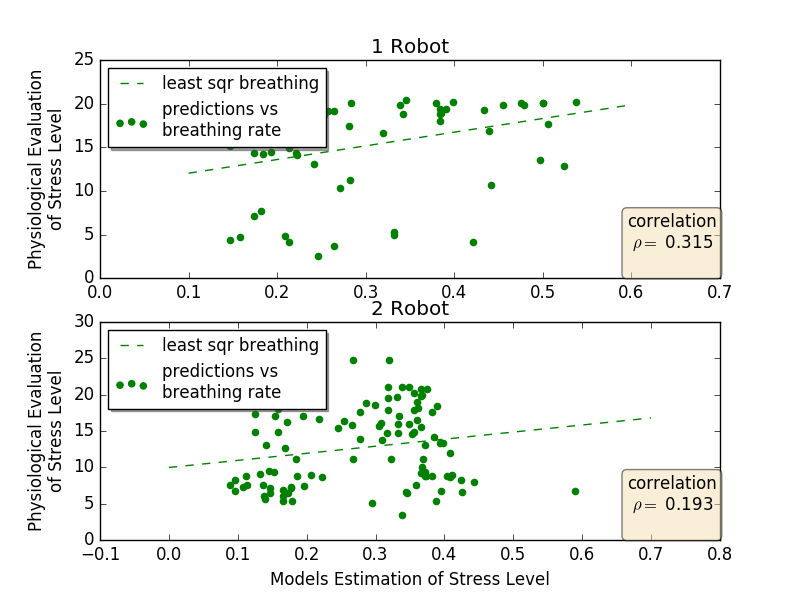
\includegraphics[width=.5\textwidth]{prediction_vs_b_p_2.png}
\caption{Robot's estimated cognitive stress level modestly correlates
  with physiological metrics.}
\label{fig:pred_phy}
\end{figure}

\begin{figure}
\centering
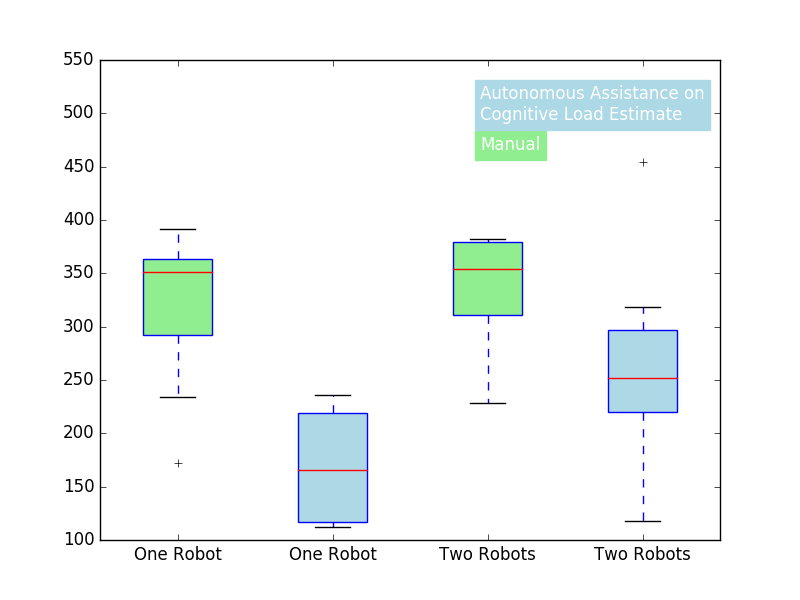
\includegraphics[width=.5\textwidth]{BoxWiskerTimesCompMaualVsAuto2.png}
\caption{Coin game task penalties in manual vs. autonomous assistance
  modes across 34 test subjects. $p < 0.05$ in both instances.}
\label{fig:BoxWiskersTimeComp}
\end{figure}

%Fig~\ref{fig:coder_eval_1_2}.
%% From our experiments we have found that
%% the cognitive load estimate from the robots using our model correlates
%% with the coder evaluated stress level by a factor $\rho=.205$ and
%% $\rho=.25$ for coin game played with one and two robots
%% respectively. Our experiment also captures that posture and breathing
%% rate of human operator as objective metric for estimating cognitive
%% stress level.We could not find any interesting pattern in other
%% physiological objective metrics i.e. heart rate, ECG amplitude using
%% our model and experimental setup.The benefits of this can be seen in
%% Fig~\ref{fig:BoxWiskersTimeComp}.  It is critical for interpreting the
%% information in Fig.
%% %\ref{fig:coder_eval_1_2} or
%% \ref{fig:pred_phy} to
%% note that while the robot's cognitive load evaluation and the scoring
%% technique for quantifying self-reported user stress both produce a
%% result between zero and one \textit{their magnitudes are not directly
%%   comparable}.Whenever cognitive stress occurs or changes, the robot
%% is able to recognize this increase for most cases in the tested
%% scenarios, and the robot's evaluation agrees with self-reported user
%% stress.

%% \begin{table}[]
%%   \centering
%%   \caption{Task success comparisons between autonomous assistance mood
%%     and manual mood.}
%%   \label{tab:task_success}
%%   \begin{tabular}{@{}|c|c|c|c|c|@{}} \toprule Game Mode & \multicolumn{2}{c|}{Manual} &
%%     \multicolumn{2}{c|}{\begin{tabular}[c]{@{}c@{}}Autonomous
%%     \\ Assistance on high\\ Stress level\end{tabular}} \\ \midrule
%%     \begin{tabular}[c]{@{}c@{}}Number of\\ Robots\\ Participated\end{tabular} & one     & two  & one  & two  \\ \midrule
%%       \begin{tabular}[c]{@{}c@{}}Number of Failure/\\ Total Number\\ of Game Played\end{tabular} & 3/7 & 3/7 & 0/10 & 1/10 \\
%%         \midrule \begin{tabular}[c]{@{}c@{}}Task Success Score\\ per game\end{tabular}                & 318  & 355  & 170  &
%%           258.2   \\ \bottomrule \end{tabular} 
%% \end{table}

%% \begin{figure}
%% \centering
%% 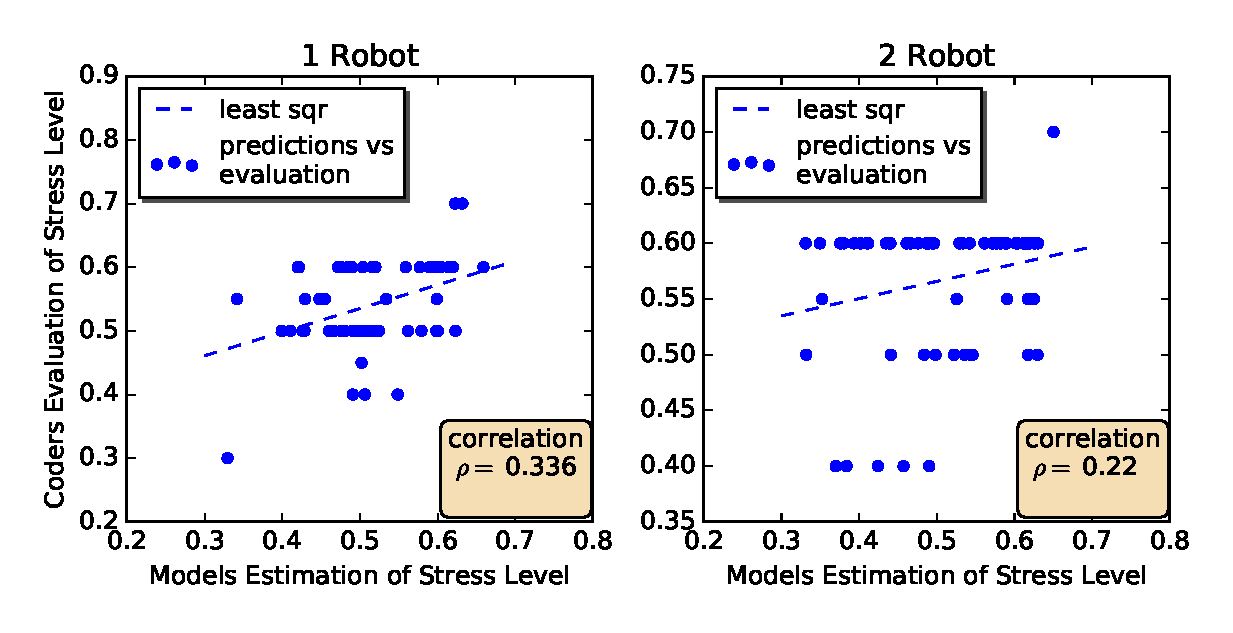
\includegraphics[width=.5\textwidth]{coder_eval_1_2.eps}
%% \caption{Cognitive load of human operators in Coin Game experiments
%%   with differing numbers of robots and steadily increasing task
%%   complexity.}
%% \label{fig:coder_eval_1_2}
%% \end{figure}


\section{Conclusion}

Robots that are capable of understanding the cognitive load their
operator is experiencing are vital to safe and efficient teamwork in
complex scenarios where the proper level of autonomy and interaction
is fluid.  Vital communication cues are embedded in the way we behave
in particular circumstances, and these implicit indicators do not have
to be lost on our robots.  Our work's contribution is to demonstrate a
quantitative, learnable, generalizable model that allows a robot to
determine that a user has succumbed to cognitive stress, even when it
cannot independently assess the instructions it is being given.

This work was supported by NSF award \#1539070 (Unmanned Aircaft
System for Atmospheric Physics).

\bibliographystyle{abbrv}
%\bibliographystyle{acmlarge}
\bibliography{sigproc-2}

\end{document}
